% Prefer the assignment's Elsevier CAS class when available; fall back to a
% portable article layout in environments without cas-sc.cls.
\IfFileExists{cas-sc.cls}{\documentclass[a4paper,fleqn]{cas-sc}}{\documentclass[a4paper,11pt]{article}}
\usepackage[margin=25mm]{geometry}
\usepackage[T1]{fontenc}
\usepackage[utf8]{inputenc}
\usepackage{lmodern}
\usepackage{microtype}
\usepackage{graphicx}
\usepackage{booktabs}
\usepackage{longtable}
\usepackage{array}
\usepackage{hyperref}
\usepackage{xcolor}
\usepackage{enumitem}
\usepackage{caption}
\hypersetup{colorlinks=true,linkcolor=blue,citecolor=blue,urlcolor=blue}
\graphicspath{{figures/}}
\setlength{\parskip}{0.45em}
\setlength{\parindent}{0pt}
\title{SAT Encodings for Sudoku: Implementation and Benchmark Study}
\author{[ADD AUTHOR NAME]\\[ADD STUDENT ID]\\[ADD AFFILIATION]}
\date{Assignment 1 -- Modern Problems in Computer Science}
\begin{document}
\maketitle

\begin{abstract}
This report describes a Sudoku solver that constructs a conjunctive normal form (CNF) formula and solves it with SAT solvers exposed by PySAT. The implementation supports eight at-most-one (AMO) encodings, optional redundant at-least-one (ALO) constraints for units, solution decoding, and independent validation. The committed benchmark snapshot contains 527 rows: SAT and baseline solving on 9$\times$9 through 36$\times$36 grids, and encoding-only measurements through 64$\times$64. The tracked instances use three generated puzzles per size at a 0.4 clue keep ratio and do not check uniqueness. We report descriptive counts and formula sizes, distinguish solve outcomes from encoding-only rows, and avoid ranking encodings from this small, unpartitioned legacy sample. The repository also contains benchmark tooling for more reproducible future runs; its newer local schema-v3 results are untracked and are not used here.
\end{abstract}

\textbf{Keywords:} Sudoku; SAT; CNF; PySAT; cardinality constraints; benchmark reproducibility

\section{Introduction}
Sudoku is a finite constraint satisfaction problem. For a grid of side length $N=b^2$, each cell receives one of $N$ symbols, and every row, column, and $b\times b$ box contains each symbol exactly once. This project studies a propositional encoding of those constraints and compares SAT solving with exact CP and MIP baselines where the local environment permitted runs.

Assignment 1 asks students to implement a solver for Sudoku or N-Queens using SAT solvers through PySAT, conduct experiments including large matrices, compare SAT with exact alternatives including CPLEX CP, CPLEX MIP, Gurobi, and CP-SAT, and present the work as a scientific-style paper with a source/results repository link in Data Availability. The assignment encourages AMO/ALO encodings such as binary, commander, product, and sequential counter. The accompanying sample is used only for paper structure; its 2DBMP topic and claims do not apply to Sudoku. The assignment lists an Elsevier CAS LaTeX class as an example. That class file was not present in the repository or local TeX installation when this source was prepared; this document therefore uses a portable article layout pending author/instructor confirmation.

\section{Sudoku model and CNF encoding}
\subsection{Variables and constraints}
For each row $r$, column $c$, and value $v$ in $\{1,\ldots,N\}$, the encoder defines a Boolean variable $x_{r,c,v}$, true when cell $(r,c)$ contains $v$. The primary variable identifiers occupy $1$ through $N^3$; auxiliary variables used by cardinality encodings are allocated after them. Each cell has an exactly-one constraint over its $N$ value variables. For each value, each row, column, and box has an at-most-one constraint. Given clues are represented by unit clauses. The implementation can additionally emit an at-least-one clause for each row/value, column/value, and box/value group; these unit ALO clauses are controlled by the \texttt{unit\_alo} option and are redundant given the cell exactly-one and unit AMO constraints. Cell ALO clauses remain required.

\subsection{AMO and ALO encodings}
The repository implements \texttt{pairwise}, \texttt{sequential}, \texttt{commander}, \texttt{binary}, and \texttt{product} AMO encodings in \texttt{src/encodings/amo.py}. The commander family has published CNF applications [2]. It also exposes PySAT-generated \texttt{pysat\_seqcounter}, \texttt{pysat\_bitwise}, and \texttt{pysat\_ladder} through the PySAT toolkit [1]. ALO is a single positive clause containing the group variables (\texttt{src/encodings/alo.py}). The repository tests check AMO behavior exhaustively over selected group sizes: all assignments with at most one true input remain satisfiable, while assignments with any pair of true inputs are rejected. This is implementation-level evidence, not a formal proof of every possible auxiliary assignment.

\subsection{Solving, decoding, and validation}
The materialized solver path builds a CNF and passes it to a PySAT solver. A newer streaming path can generate clauses directly into a solver while preserving the same encoding semantics; streaming is an implementation capability and was not the path used to produce the committed schema-v1 result rows. A satisfying assignment is decoded using the primary cell variables. Decoded grids are validated against grid dimensions, value ranges, original clues, and all row, column, and box constraints before a benchmark row is marked valid. Optional uniqueness checking blocks the selected cell assignment and solves again; UNSAT on the blocked formula indicates uniqueness. The committed benchmark did not enable this check.

\section{Implementation and experimental setup}
\subsection{Repository and solvers}
The repository contains a command-line entry point, puzzle I/O and validation, the encoder and solver, a benchmark harness, plotting/audit utilities, tests, and baseline adapters. SAT benchmark rows use CaDiCaL 1.9.5, Glucose 4.2, Kissat 4.0.4, and MiniSat 2.2 (PySAT solver identifiers: \texttt{cadical195}, \texttt{glucose42}, \texttt{kissat404}, \texttt{minisat22}). The requested exact baselines are represented by CP-SAT, Gurobi, CPLEX MIP, and CPLEX CP; CBC ILP is an additional baseline. In the committed data, some Gurobi and CPLEX outcomes are recorded as \texttt{license\_limit}. These are reported as recorded outcomes, not inferred timeouts or solver failures. Whether a different academic or commercial license would remove each limit requires a run with that license.

\subsection{Committed data snapshot}
The report uses \texttt{results/results.csv}, the tracked schema-v1 file, with 527 rows and 17 columns. Its first recorded run used a 60-second requested timeout, three puzzles per box size, a 0.4 clue keep ratio, and sizes 9, 16, 25, and 36 for solving. Puzzle seeds followed the legacy rule $1000b+i$ (where $b$ is box size and $i$ is the puzzle index). Rows for sizes 49 and 64 are encoding-only. The size table has no pairwise count at 64 because that encoding was skipped for the largest size due to memory constraints. The data do not record uniqueness checks; generated puzzles have at least one solution inherited from a completion, but uniqueness is not guaranteed.

The metadata records Python 3.14.4 and platform details for the run; the recorded source commit is \texttt{0dcf16efbbcd005328ce590fe2611af262343f23}. CI targets Python 3.12. The current benchmark code and README describe richer schema-v4 provenance and timing semantics, but those guarantees must not be retroactively attributed to the committed schema-v1 CSV. A separate 3,753-row schema-v3 file exists only as an untracked local artifact and is excluded from the results below.

\begin{table}[ht]
\centering
\caption{Recorded outcome counts in the committed schema-v1 CSV. Rows count method/solver executions, not distinct puzzles.}
\begin{tabular}{lrr}
\toprule
Outcome & Count & Interpretation \\
\midrule
Solved & 444 & Includes SAT and exact baseline rows \\
Timeout & 13 & Recorded timeout status \\
License limit & 23 & Recorded baseline license-limit status \\
Encoded & 47 & Formula-size experiment; no solver call \\
\midrule
Total & 527 & All rows in the tracked CSV \\
\bottomrule
\end{tabular}
\end{table}

The 47 encode-only rows cover 9, 16, 25, 36, 49, and 64. Solving rows occur only at 9 through 36. Within the 60 baseline rows, CP-SAT solved 12; CBC solved 7 and timed out 5; CPLEX CP solved 7 and recorded 5 license-limit outcomes; CPLEX MIP solved 3 and recorded 9 license-limit outcomes; Gurobi solved 3 and recorded 9 license-limit outcomes. These counts describe this environment and sample only.

\section{Results}
\subsection{Solving outcomes and limits}
The schema-v1 audit reports 444 solved rows and confirms that all 444 have \texttt{valid=True}. The existing audit also re-verifies 132 saved/generated puzzle records against their seeds and hashes. This is evidence for the recorded instances and validator path. It does not establish uniqueness, generalize to untested puzzles, or replace independent replication.

Figure~\ref{fig:baselines} visualizes available SAT/baseline outcomes from the canonical CSV. Because the sample has only three puzzles per size, one clue density, legacy unpartitioned configuration selection, timeouts, and license-limited cells, it is descriptive. No method is declared fastest. In particular, configurations selected using the same evaluation instances cannot support an unbiased performance ranking.

\begin{figure}[ht]
\centering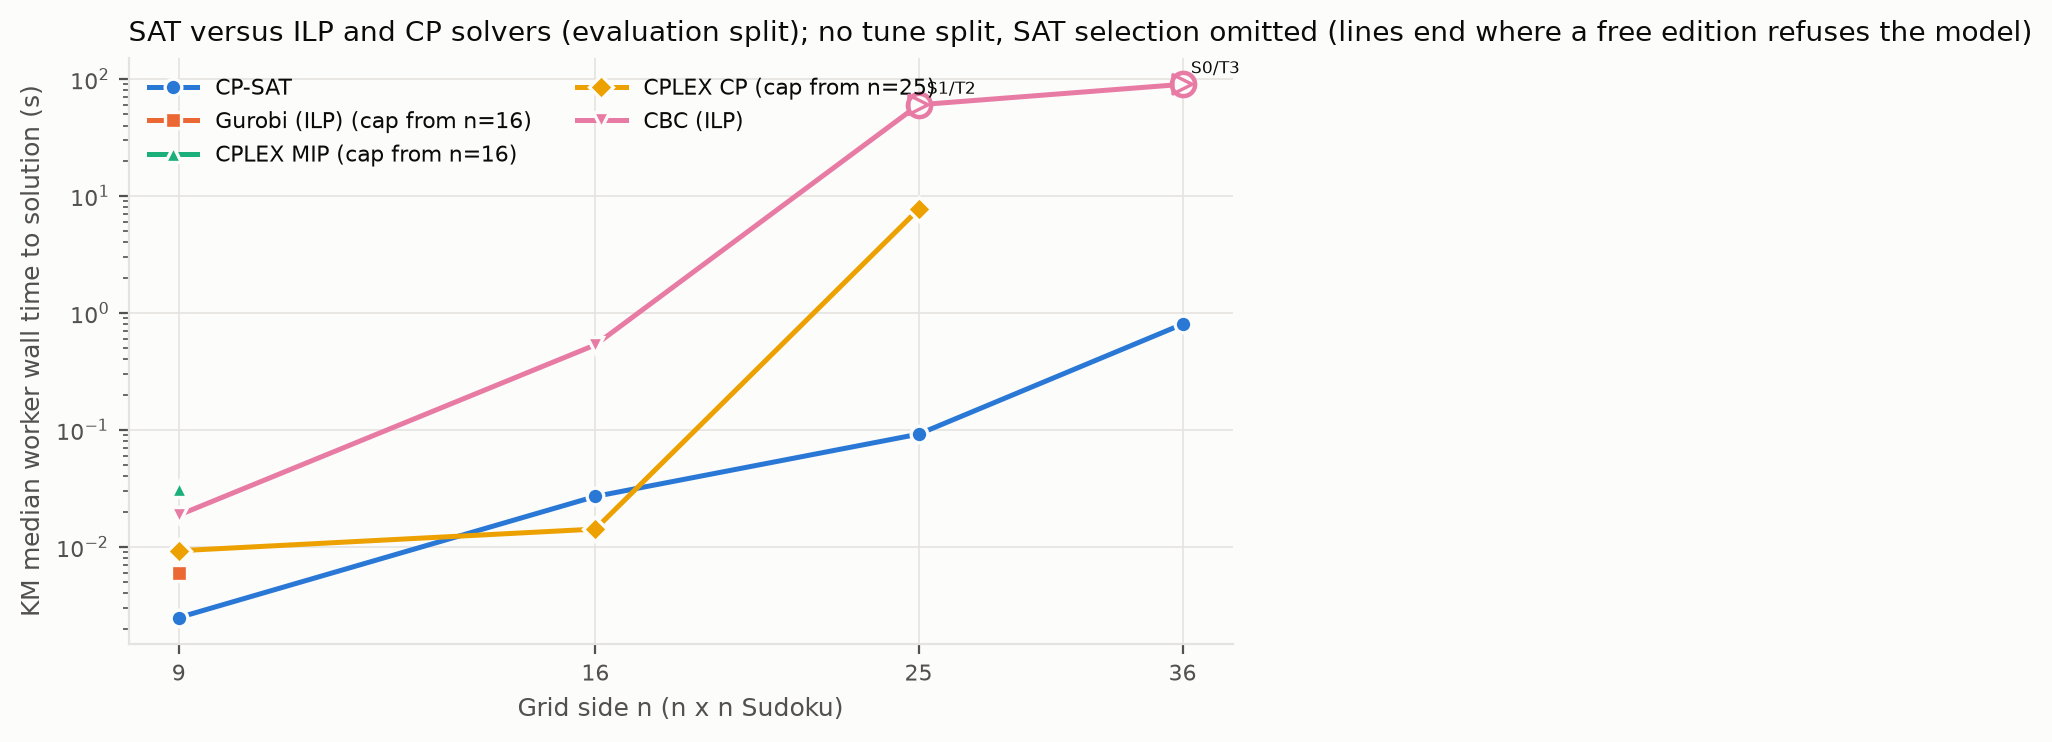
\includegraphics[width=0.94\linewidth]{fig_vs_baselines.png}
\caption{Existing baseline comparison figure generated from the tracked schema-v1 CSV. It is descriptive; license caps and timeouts remain distinct outcomes.}\label{fig:baselines}
\end{figure}

\subsection{Encoding size}
Figure~\ref{fig:size} and Table~\ref{tab:size} describe formula size in variables and clauses. For example, at $N=36$, pairwise has 3,271,602 clauses and 46,656 variables, while product has 534,450 clauses and 108,864 variables. At $N=64$, the recorded product formula has 2,836,149 clauses and 720,896 variables. These are encoding-size measurements only: fewer clauses or variables do not by themselves imply shorter solving time or lower peak memory. No size experiment at 49 or 64 solved the resulting formula.

\begin{figure}[ht]
\centering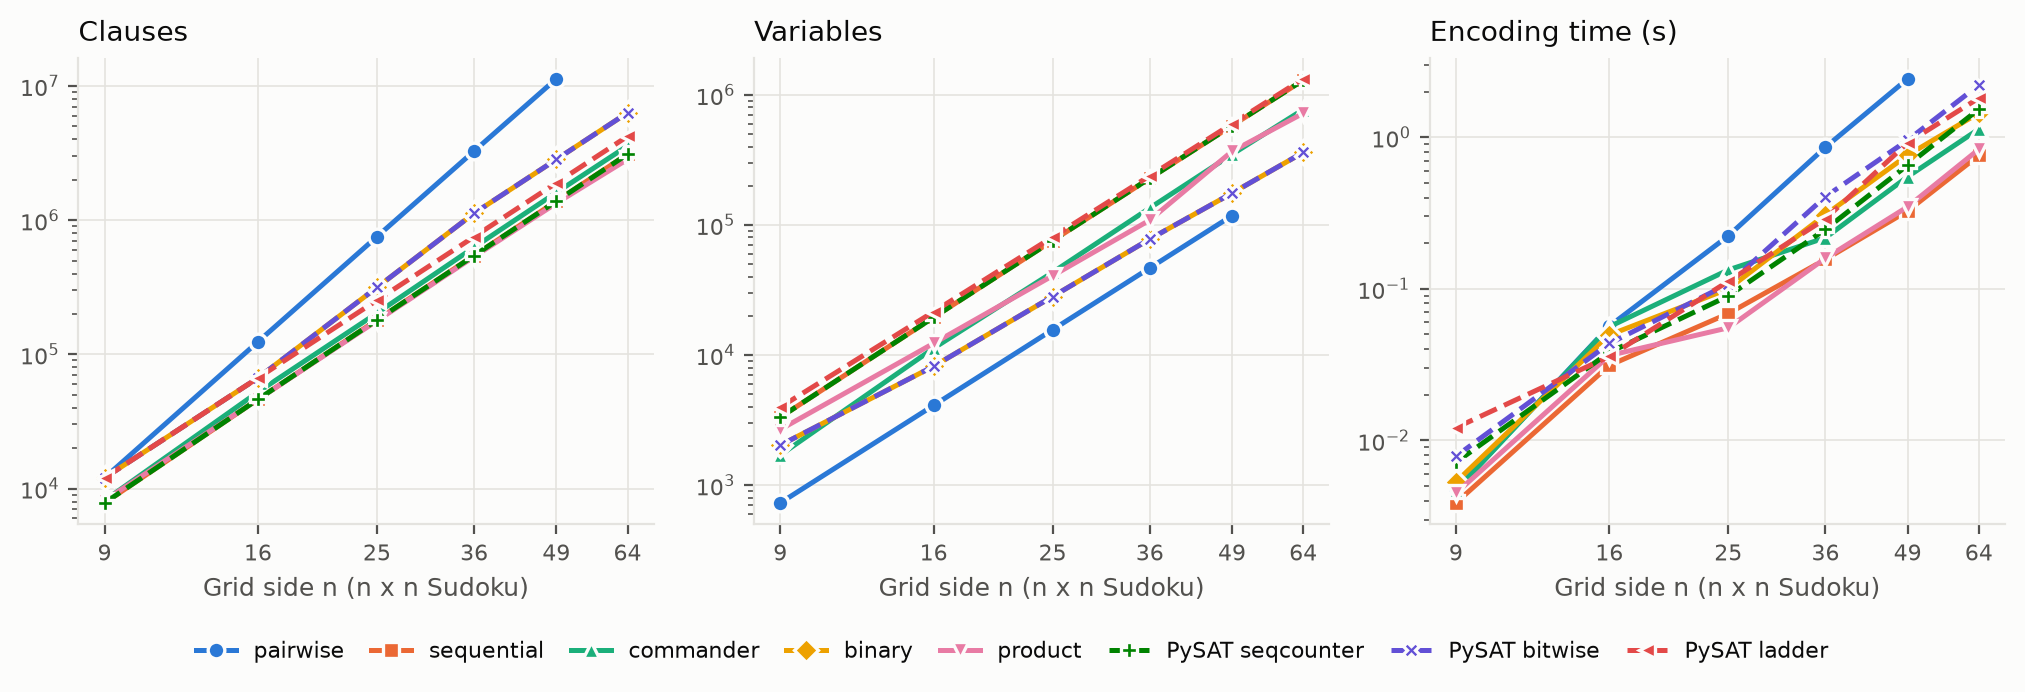
\includegraphics[width=0.88\linewidth]{fig_encoding_size.png}
\caption{Existing encoding-size figure, based on the canonical result set. Encoding-only observations are not solving results.}\label{fig:size}
\end{figure}

\begin{table}[ht]
\centering
\caption{Selected clause counts from the existing size table. These counts do not rank solving speed.}\label{tab:size}
\begin{tabular}{rrrr}
\toprule
Grid & Pairwise clauses & Sequential clauses & Product clauses \\
\midrule
9 & 12,020 & 7,808 & 8,132 \\
16 & 124,024 & 46,200 & 46,200 \\
25 & 752,749 & 180,249 & 177,749 \\
36 & 3,271,602 & 544,818 & 534,450 \\
49 & 11,304,899 & 1,383,967 & 1,335,947 \\
64 & -- (skipped) & 3,098,293 & 2,836,149 \\
\bottomrule
\end{tabular}
\end{table}

\begin{figure}[ht]
\centering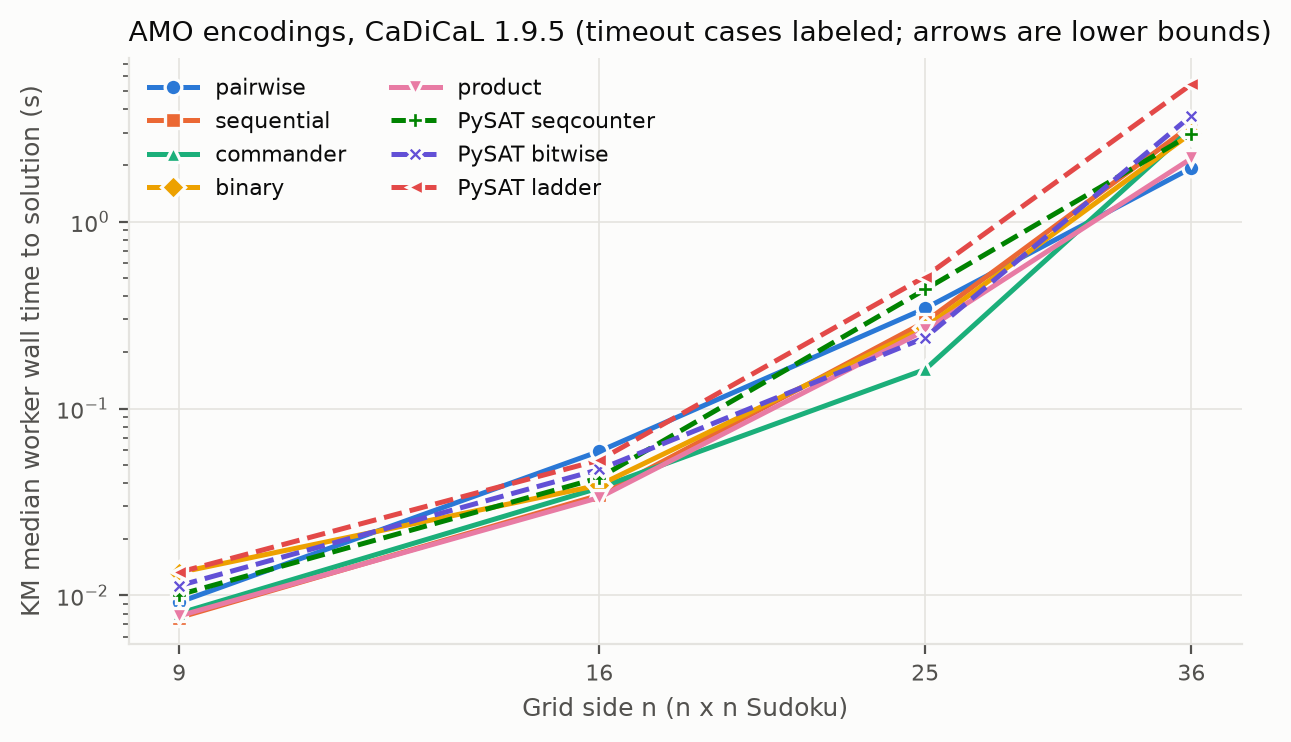
\includegraphics[width=0.91\linewidth]{fig_amo_vs_n.png}
\caption{Existing AMO result visualization for solved sizes. The small legacy sample is insufficient for a general encoding-speed claim.}\label{fig:amo}
\end{figure}

\section{Reproducibility and threats to validity}
The current benchmark tooling supports explicit seeds and clue densities, shared puzzle identity across methods, append/resume behavior, separate outcome states, timing phases, and an audit command. The committed v1 CSV predates much of that row-level provenance: it lacks the later per-row run/configuration/puzzle hashes and split metadata. The tracked \texttt{results/meta.json} contains run-level settings, but its later schema-v3 run refers to an untracked local result file. The audit command for the selected data is:
\begin{verbatim}
MPLCONFIGDIR=/tmp/sudoku-mpl-cache .venv/bin/python -m src.plot_results \\
  --csv results/results.csv --out results --audit
\end{verbatim}
The audited snapshot reports schema v1 valid, 527 rows, all solved rows valid, and the saved puzzle records passing seed/hash checks.

Primary validity limits are: three instances per size; one clue density; no uniqueness test; a single recorded run/environment; legacy tuning/evaluation overlap; limited solve sizes; and solver license constraints. Timeouts and license limits reduce the set of comparable completed runs. Formula-size measurements at large grids must not be interpreted as solving scalability. Figures and tables included here are existing artifacts checked against the canonical CSV; the newer local v3 CSV was not used.

\section{Conclusion}
The repository demonstrates an end-to-end Sudoku-to-CNF implementation with multiple AMO choices, PySAT solving, exact-solver adapters, solution validation, and reproducibility-oriented tooling. The committed results establish that the tested SAT and baseline configurations solved many generated instances through 36$\times$36, while the 49$\times$49 and 64$\times$64 data establish encoding construction only. The current evidence supports descriptive reporting of outcomes and formula sizes, not a robust claim that one encoding or solver is fastest. A stronger follow-up should use more seeds and clue densities, a held-out evaluation split, shared puzzle records, explicit timeout/memory accounting, and licensed/available solver environments.

\section*{Data Availability}
Source code, tests, the example puzzle, the tracked raw benchmark file \texttt{results/results.csv} (schema v1), metadata, saved instances, and the figures and tables used in this report are present in this repository checkout. The report source is \texttt{report/main.tex}; the compiled report is \texttt{main.pdf}. The schema-v3 CSV mentioned in metadata is an untracked local file and is not claimed as published data. The configured Git remote is \url{https://github.com/canknotcawh/sudoku_sat_solver}, while the prior README contains \url{https://github.com/canknotcaw/sudoku_sat_solver}; the official repository URL cannot be established from this checkout and requires author confirmation. No repository or data license is asserted here.

\section*{Declarations}
\textbf{Author contributions:} [AUTHOR TO PROVIDE CONTRIBUTIONS].\\
\textbf{Competing interests:} [AUTHOR TO CONFIRM].\\
\textbf{Funding:} [AUTHOR TO CONFIRM].\\
\textbf{Acknowledgements:} [AUTHOR TO PROVIDE OR REMOVE].\\
\textbf{Integrity statement:} [AUTHOR TO PROVIDE ANY REQUIRED COURSE DECLARATION].\\
\textbf{AI use statement:} [AUTHOR TO CONFIRM REQUIRED DISCLOSURE].

\section*{References}
\begin{enumerate}[leftmargin=*]
\item A. Ignatiev, A. Morgado, and J. Marques-Silva. PySAT: A Python toolkit for prototyping with SAT oracles. In \emph{SAT}, 2018. DOI: \href{https://doi.org/10.1007/978-3-319-94144-8_26}{10.1007/978-3-319-94144-8\_26}.
\item W. Klieber and G. Kwon. Efficient CNF encoding for selecting 1 from N objects. 2007. Available at \url{https://www.cs.cmu.edu/~wklieber/papers/2007_efficient-cnf-encoding-for-selecting-1.pdf}.
\item Google OR-Tools. CP-SAT solver documentation. \url{https://developers.google.com/optimization/cp/cp_solver}.
\item Gurobi Optimization, LLC. Numeric codes documentation. \url{https://docs.gurobi.com/projects/optimizer/en/current/reference/numericcodes.html}.
\end{enumerate}

\appendix
\section{Author completion checklist}
Before submission, replace all bracketed placeholders; verify the official GitHub URL and repository visibility; confirm author identity and institutional details; provide required contribution, integrity, funding, acknowledgement, competing-interest, and AI-use statements; add any encoding literature required by the instructor; and confirm whether the CAS class is mandatory. Confirm that the final report and source are committed/published before claiming public availability. The repository does not contain evidence to fill these fields.
\end{document}
